%%% LaTeX Template: Two column article
%%%
%%% Source: http://www.howtotex.com/
%%% Feel free to distribute this template, but please keep to referal to http://www.howtotex.com/ here.
%%% Date: February 2011

%%% Preamble
\documentclass[	DIV=calc,%
							paper=a4,%
							fontsize=12pt,%
							onecolumn]{scrartcl}	 					% KOMA-article class

\usepackage{lipsum}													% Package to create dummy text
\usepackage[brazil]{babel}										% English language/hyphenation
\usepackage[protrusion=true,expansion=true]{microtype}				% Better typography
\usepackage{amsmath,amsfonts,amsthm}					% Math packages
\usepackage[pdftex]{graphicx}									% Enable pdflatex
\usepackage[svgnames]{xcolor}									% Enabling colors by their 'svgnames'
\usepackage[hang, small,labelfont=bf,up,textfont=it,up]{caption}	% Custom captions under/above floats
\usepackage{epstopdf}												% Converts .eps to .pdf
\usepackage{subfig}													% Subfigures
\usepackage{booktabs}												% Nicer tables
\usepackage{fix-cm}													% Custom fontsizes
\usepackage{float}
\usepackage[utf8]{inputenc}
\usepackage[top=2.5cm, bottom=2.5cm, left=2.5cm, right=2.5cm]{geometry}
\usepackage[ddmmyyyy]{datetime}
\addto\captionsenglish{%
	\renewcommand\tablename{Tabela}
	\renewcommand\figurename{Figura}
} 
 

 
%%% Custom sectioning (sectsty package)
\usepackage{sectsty}													% Custom sectioning (see below)
\allsectionsfont{%															% Change font of al section commands
	\usefont{OT1}{phv}{b}{n}%										% bch-b-n: CharterBT-Bold font
	}

\sectionfont{%																% Change font of \section command
	\usefont{OT1}{phv}{b}{n}%										% bch-b-n: CharterBT-Bold font
	}



%%% Headers and footers
\usepackage{fancyhdr}												% Needed to define custom headers/footers
	\pagestyle{fancy}														% Enabling the custom headers/footers
\usepackage{lastpage}	

% Header (empty)
\lhead{}
\chead{}
\rhead{}
% Footer (you may change this to your own needs)

%% ====================================
%% ====================================
%% mude o rodape  do projeto
%% ====================================
%% ====================================

\lfoot{\footnotesize \texttt{Cabeamento estruturado} \textbullet ~Modelo de projeto}


\cfoot{}
\rfoot{\footnotesize página \thepage\ de \pageref{LastPage}}	% "Page 1 of 2"
\renewcommand{\headrulewidth}{0.0pt}
\renewcommand{\footrulewidth}{0.4pt}



%%% Creating an initial of the very first character of the content
\usepackage{lettrine}
\newcommand{\initial}[1]{%
     \lettrine[lines=3,lhang=0.3,nindent=0em]{
     				\color{DarkGoldenrod}
     				{\textsf{#1}}}{}}



%%% Title, author and date metadata
\usepackage{titling}															% For custom titles

\newcommand{\HorRule}{\color{DarkGoldenrod}%			% Creating a horizontal rule
									  	\rule{\linewidth}{1pt}%
										}

\pretitle{\vspace{-30pt} \begin{flushleft} \HorRule 
				\fontsize{50}{50} \usefont{OT1}{phv}{b}{n} \color{DarkRed} \selectfont 
				}

%% ====================================
%% ====================================
%% mude o titulo  do projeto
%% ====================================
%% ====================================

\title{Projeto de Cabeamento Estruturado - Escritório de Contabilidade RN}					% Title of your article goes here

%% ====================================



\posttitle{\par\end{flushleft}\vskip 0.5em}

\preauthor{\begin{flushleft}
					\large \lineskip 0.5em \usefont{OT1}{phv}{b}{sl} \color{DarkRed}}
\author{Nivorley de Lima Simião, Renan Barboza dos Santos}  	% Author name goes here


\postauthor{\footnotesize \usefont{OT1}{phv}{m}{sl} \color{Black} 
					\\Universidade Tecnológica Federal do Paraná - Câmpus Cornélio Procópio 								% Institution of author
					\par\end{flushleft}\HorRule}

\date{}																				% No date




%%% Begin document
\begin{document}
\maketitle
\thispagestyle{fancy} 	
\thispagestyle{empty}		% Enabling the custom headers/footers for the first page 
% The first character should be within \initial{}




%% ====================================
%% ====================================
%% mude o resumo  do projeto
%% ====================================
%% ====================================
\initial{E}\textbf{ste projeto tem a intenção de propor uma reestruturação da rede de dados do Escritório de Contabilidade RN. Contempla um levantamento da situação atual, incluindo seus ativos e passivos, planta física e lógica, e apresenta uma proposta de cabeamento estruturado dentro das normas, abrangendo os itens citados anteriormente bem como levantamento de quantidade/custo, plano de certificação e orçamento.}

%% ====================================
\begin{figure}
	\centering
	\includegraphics{utfpr}
\end{figure}

\vspace{3cm}
\centerline{\textit{\textbf{\today}}}

\clearpage
    \renewcommand*\listfigurename{Lista de figuras}
\listoffigures

\renewcommand*\listtablename{Lista de tabelas}
\listoftables




\clearpage
\renewcommand{\contentsname}{Sumário}
\tableofcontents
\clearpage

%% ====================================
%% ====================================
%% Inicio do texto
%% ====================================
%% ====================================
\section{Introdução}
O objetivo desse projeto é criar uma infraestrutura de rede para o escritório de contabilidade fictício, o qual foi denominado RN, possibilitando a organização e restruturação da rede atual, a qual conta com equipamentos e instalações inadequadas, causando problemas como indisponibilidade, perda de dados, e lentidão excessiva em seus processos. 
Atualmente cerca de vinte (20) usuários compõem a equipe de funcionários ativos na rede, há também 3 (três) impressoras, 1(um) ponto de acesso sem fio, 1 (um) servidor e 1(um) roteador.
Com base nas necessidades, o projeto irá priorizar pela organização, padronização e aquisição de equipamentos condizentes com a realidade e compatíveis com futuras melhorias, levando sempre em consideração o melhor custo e benefício. 

\subsection{Benefícios}

\begin{itemize}
	\item A aquisição de novos equipamentos e a padronização das instalações tornará a rede bem mais estável;
	\item As conexões serão identificadas agilizando manutenções futuras e tornando problemas mais específicos;
	\item O novo plano de internet fibra óptica trará mais desempenho para os processos que dependem de acesso via web;
	\item A organização do cabeamento trará aos usuário e clientes uma sensação de conforto e confiança, uma vez que, a exposição dos cabos gerava problemas diários; 
	\item Facilidade na ativação de novos pontos de rede;
\end{itemize}

\section{Estado atual}
A rede atualmente possui vinte e nove pontos de acesso, e a sua expansão se deu de forma desordenada, desconsiderando qualquer tipo de regra de cabeamento estruturado, desde seu início a dez anos atrás quando apenas dez máquinas faziam uso dos recursos disponíveis. Recentemente a empresa adquiriu um switch de 16(dezesseis) portas gerenciável porém, ainda utiliza dois hubs de 16(dezesseis) portas em sua estrutura, 3 (três) impressoras de rede.

\begin{itemize}
	\item Passivos de rede atuais: Cabos par trançado categoria 5E sem blindagem, conectores rj45, 2 (dois) hubs de 16(dezesseis) portas. 
	\item Ativos de rede atuais: 1(um) switch 24(vinte e quatro) portas, roteador, 1 único ponto de acesso wireless de uso residencial.
	
As principais reclamações dos usuários são: Má organização dos cabos, lentidão ao transferir arquivos entre os computadores, queda da conexão durante a execução dos processos, problemas de lentidão quando vários usuários se conectam à rede sem fio.
Analisando a rede verificou-se que a mesma não atende o requisitos mínimos para um funcionamento adequado, pois o cabeamento, conexões e estrutura física de modo geral, é realizada por pessoal não capacitado, com passivos de baixa qualidade, sem nenhuma certificação.

\end{itemize}

\section{Usuários e Aplicativos}
Todos os usuários utilizam o sistema ERP, utilizam o acesso à internet, serviços de impressão via rede. A empresa tem 4 (quatro) contadores, 12 (doze) auxiliares administrativos, 1 (um) recepcionista, 1 (um) gerente e 2 (dois) atendentes de clientes.
 

\subsection{Usuários}
Nesta empresa todos os usuários possuem perfis de administrador local, pois não há um controlador de domínios na rede, apenas um servidor de banco de dados e do sistema ERP. 

\subsection{Aplicativos}
O sistema da empresa envolve módulos de contabilidade, módulos de recursos humanos, cadastro de clientes, gerenciador de e-mails e agenda. Além disso, o contato com os clientes e realizado através do e-mail, incluindo pedidos de serviço e transferência de documentos, o que exige estabilidade da rede e do acesso à internet.


\section{Estrutura predial existente}

A estrutura predial se divide em: Uma sala da gerência, uma sala do administrativo e contabilidade e uma sala para recepção e atendimento aos clientes. O servidor se encontra na mesma sala do pessoal do administrativo. Na sala de recepção e atendimento há três computadores, um no balcão de atendimento e os outros dois, cada um em uma mesa; na sala da gerencia, há um computador e um impressora, na sala contábil e administrativo há seis ilhas de quatro lugares, distribuídas em um espaço quarenta e nove metros quadrados e em um canto dessa sala fica localizado o servidor e a impressora. Por não haver tubulação preexiste na parede e no piso os cabos ficam distribuídos através de canaletas ou até mesmo expostos.



\begin{figure}[H]
	No layout da planta pode-se verificar os setores existentes atualmente.
	\centering
	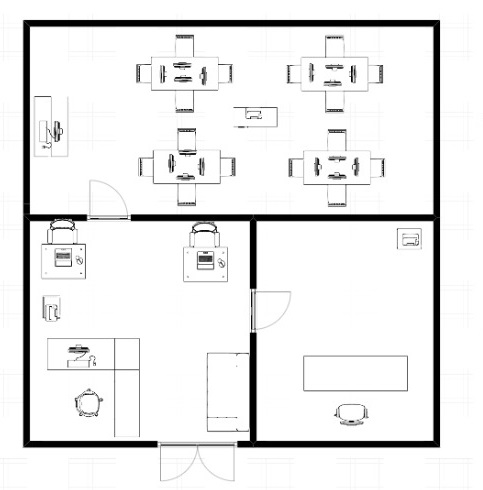
\includegraphics[scale=1]{fig1}
	\caption{Planta Baixa}
	\label{fig1}
	\end{figure}

\section{Planta Lógica - Elementos estruturados}


\begin{figure}[H]
	Equipamentos e suas devidas ligações lógicas
	\centering
	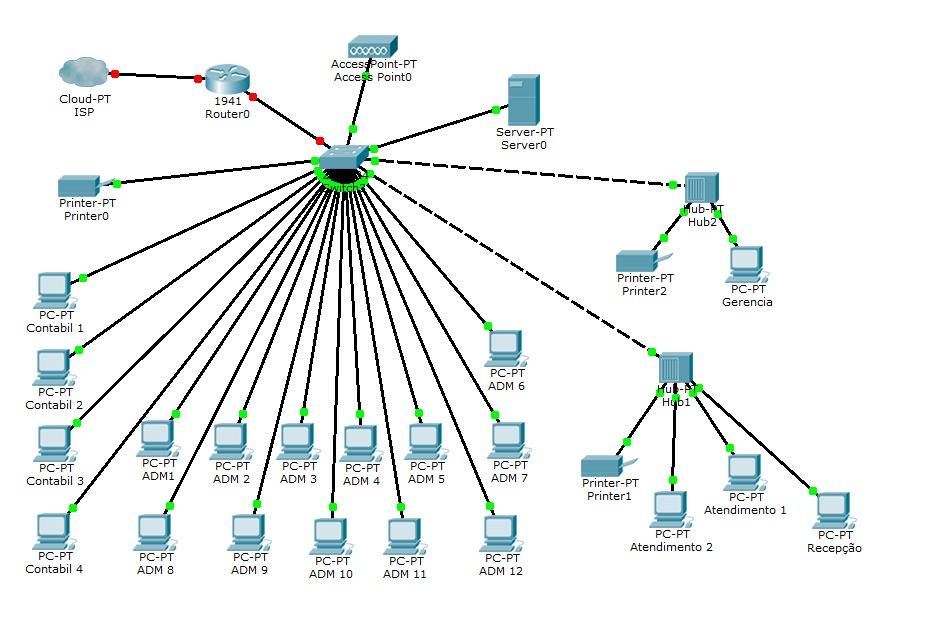
\includegraphics[scale=0.5]{fig2}
	\caption{Planta lógica}
	\label{fig2}
	\end{figure}
	

A tabela a seguir representa a distribuição dos endereços Ips para cada equipamento. Utilizando uma rede /24 (vinte e quatro) tendo em vista que a rede possui um pequeno número de dispositivos conectados. Os ips foram atribuídos manualmente os seguintes dispositivos:  roteador, access point, switch, servidor e impressoras.
O range para esses dispositivos ficou entre os ips 192.168.0.1 à 192.168.0.20. Os demais computadores do escritório, estão configurados para receber ips dinamicamente assim como os usuários que fizerem uso da conexão sem fio. O DHCP oferece ips que vão de 192.168.0.21 à 192.168.0.50.
  
    \begin{figure}[H]
	\centering
	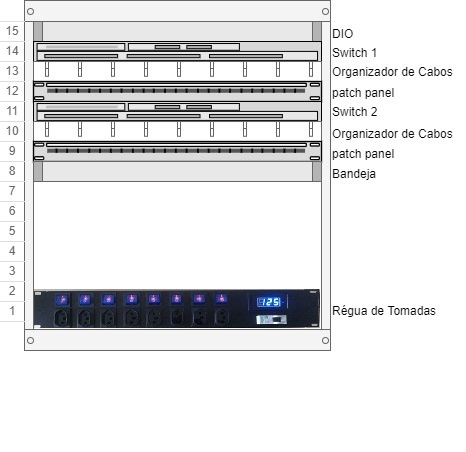
\includegraphics[scale=1]{fig5}
	\caption{Endereços de IP}
	\label{fig5}
	\end{figure}

\subsection{Diagrama de Rack}
	A figura 3 exemplifica como ficará o rack pós implantação
	\begin{figure}[H]
	\centering
	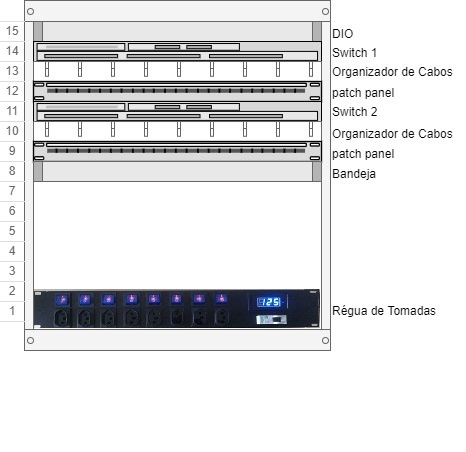
\includegraphics[scale=1]{fig3}
	\caption{Diagrama de Rack}
	\label{fig3}
	\end{figure}

\subsection{Encaminhamento}
\begin{figure}[H]
	Eletrodutos, calhas, e pontos de conexão
	\centering
	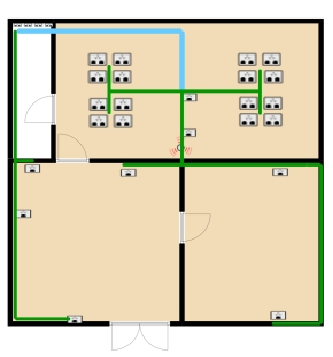
\includegraphics[scale=1.5]{fig4}
	\caption{Encaminhamento}
	\label{fig4}
	\end{figure}
	
	

\subsection{Memorial descritivo}

\begin{itemize}
	\item 2 Patch panel Standard Furukawa;
	\item 1 Rack 16U Attic;
 	\item 1 Caixa de cabo de rede CAT5E Furukawa 305m;
 	\item 1 Dio;
 	\item 60 Patch cords 1,5m Furukawa CAT5E;
 	\item 1 Bandeja de rack;
 	\item 1 Régua de tomadas de rack;
 	\item Canaletas subterrâneas;
  	 
\end{itemize}


\subsection{Identificação dos cabos}
Explique como os cabos serão identificados em seu projeto. Coloque uma relação dos cabos instalados e identificados.

\section{Implantação}
Estabeleça um cronograma de implantação:
Remoção de equipamentos existentes (destino para descarte), instalação dos condutores, instalação dos cabos, 
identificação dos cabos, montagem dos racks, certificação, etc... Crie atividades e estabeleça o tempo de execução. Se for um projeto real, indique também quais os responsáveis pela execução do projeto e de cada uma das etapas.

Defina marcas (e padrões) e fornecedores se for o caso. Atenção a contratados e subcontratados para a realização das atividades. Estabeleça a responsabilidade de execução da atividade e também da validação dela.

Utilize algum software para gerear o cronograma. Excel,etc. O fundamental é dividir em etapas, descrever e estimar o tempo de cada uma delas.

Segue uma relação de ferramentas:
http://asana.com/, 
https://trello.com/, 
http://www.ganttproject.biz/, 
http://www.orangescrum.org/. 

\section{Plano de certificação}
Quais seriam as etapas para a certificação? 
Quais os locais e horários para execução da certificação na rede? Toda rede será certificada?
Como os testes seriam executados?
Quais relatórios de certificação serão (ou deveriam ser) entregues? 

\section{Plano de manutenção}

Revisões periódicas na rede, emissão de certificados para novos pontos.

\subsection{Plano de expansão}
Existe um plano de expansão? Quantos novos pontos poderão ser acrecidos na rede, antes de migração de equipamentos na camada 2? Se houver expansão, quais equipamentos deverão ser direcionados para as estremidades da rede? 

\section{Risco}
Apresentar os riscos do projeto

\section{Orçamento}
Crie uma relação de orçamentos baseado na seções anteriores.

\section{Recomendações}
Observações e recomendações para o cliente.

\section{Referências bibliográficas}
Utilize o mendley, o jabref ou diretamente o bibtex para gerenciar suas referências biliográficas. As referências são criadas automaticamente de acordo com o uso no texto.

Exemplo: Redes de computadores, segundo \cite{t2013} é considerada..... Já \cite{kurose2010} apresenta uma versão...

Analisando os pressupostos de \cite{ref3} e \cite{ref4} concluimos que....


\renewcommand\refname{} %%Referências bibliográficas}  
\bibliographystyle{ieeetr}
\bibliography{referencias}  

\end{document}
